\chapter{Literature Survey}
\label{ch:literature}

Both works surveyed in this chapter follow the same high-level idea: perform the expensive,
precise analysis \emph{statically}, ship its results with the program, and let the JIT compiler
use them cheaply at run time. They differ in what they do about the two problems raised in
Section~\ref{sec:challenges}: PYE handles missing library code, while optimistic stack allocation
handles dynamic features that can invalidate static results.

\section{The PYE Framework}

PYE (\emph{Precise-Yet-Efficient}) by Thakur and Nandivada~\cite{thakur2019pye} is a two-stage
(static\,+\,JIT) analysis framework for Java programs. Its key contributions are:
\begin{itemize}
  \item a way to record dependences between the application and the libraries it calls,
        called \emph{conditional values};
  \item offloading the expensive part of the analysis to the static compiler, which produces
        \emph{partial summaries} expressed in terms of conditional values; and
  \item enabling highly precise analysis results that the JIT compiler can evaluate cheaply at
        run time, once the actual libraries are known.
\end{itemize}

\subsection{Architecture}

Figure~\ref{fig:pye} shows the two halves of PYE.

\begin{figure}[htbp]
  \centering
  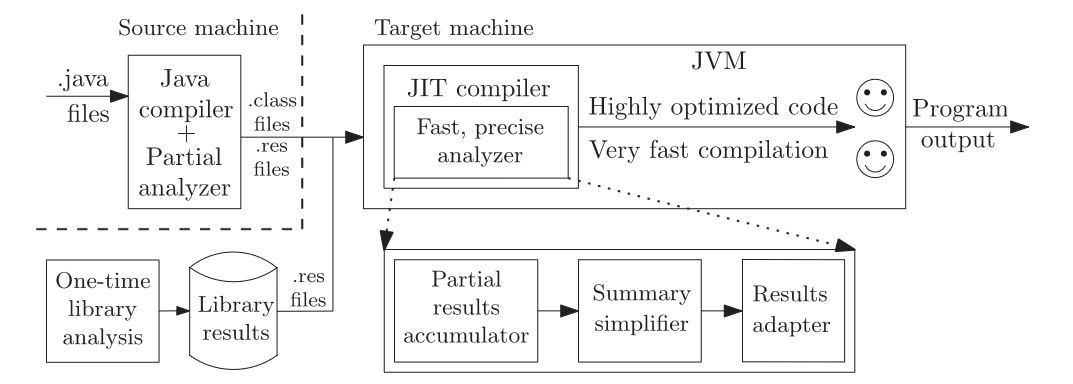
\includegraphics[width=0.9\linewidth]{figures/pye_architecture.png}
  \caption{Architecture of PYE (adapted from~\cite{thakur2019pye}). The static side writes
           partial summaries to \texttt{.res} files; the JIT side combines them with library
           summaries to obtain final results.}
  \label{fig:pye}
\end{figure}

\paragraph{Static compiler + partial analyzer.} On the source machine, PYE performs a precise
analysis of the application. Calls to library methods, whose code may not be available or may
change before the program runs, are \emph{skipped} rather than approximated. The resulting
partial summaries are written to \texttt{.res} files that ship with the \texttt{.class} files.
Library methods are analysed once, separately, in the same way.

\paragraph{JIT compiler + fast-precise analyzer.} On the target machine, when the JIT compiler
compiles a method, it reads only the summaries it needs, resolves the dependences between
application and library summaries, and populates the relevant JVM data structures with the final
results. Since all of the heavy lifting has already happened statically, this step is fast.

\subsection{Conditional Values}

A traditional summary maps each object in a method to a single data-flow value; for escape
analysis this is \textsc{Escape} or \textsc{NoEscape}. When part of the program is missing, such
a summary must be conservative. PYE's partial summaries instead map each element of a method's
domain to a \emph{set of conditional values}.

\begin{defbox}{Definition 1 (Conditional value)}
A conditional value is a triple
\[ T = \langle \Theta,\ \mathit{val},\ \mathit{val}' \rangle, \]
where
\begin{itemize}
  \item $\Theta = \langle u, x \rangle$, with $u$ a method and $x$ a program element in $u$; and
  \item $\mathit{val}, \mathit{val}' \in \mathit{Val}$, the set of values of the data-flow equations.
\end{itemize}
It reads: \emph{if element $x$ of method $u$ has value $\mathit{val}$, then the element being
summarized has value $\mathit{val}'$}.
\end{defbox}

Consider the method in Listing~\ref{lst:cv}, where \texttt{bar} is a library method that is not
available during static analysis.

\begin{minipage}[t]{0.47\textwidth}
\begin{lstlisting}[language=Java, caption={Example for conditional values.}, label={lst:cv}]
void foo(A p) {
  A a = new A();   // O1
  A b = new A();   // O2
  A c = new A();   // O3
  bar(b);          // library method
  c.g = 10;
}
\end{lstlisting}
\end{minipage}\hfill
\begin{minipage}[t]{0.48\textwidth}
\vspace{10pt}
\centering
\begin{tabular}{@{}ll@{}}
  \toprule
  Object & Conditional values \\
  \midrule
  $O_1$ & $\emptyset$ \quad (never escapes) \\
  $O_2$ & $\{\cv{\langle \mathit{bar}, p_0\rangle}{E}{E}\}$ \\
  $O_3$ & $\emptyset$ \quad (never escapes) \\
  \bottomrule
\end{tabular}
\end{minipage}

\medskip
Objects $O_1$ and $O_3$ never leave \texttt{foo}, so they need no condition. Object $O_2$ is
passed to \texttt{bar}; whether it escapes depends entirely on what \texttt{bar} does with its
first parameter $p_0$. Instead of giving up and marking $O_2$ as escaping, PYE records the
conditional value $\cv{\langle \mathit{bar}, p_0\rangle}{E}{E}$: \emph{$O_2$ escapes if and
only if $p_0$ escapes in \texttt{bar}}. At run time the JIT compiler looks up the summary of the
actual \texttt{bar}, evaluates the condition, and obtains a precise answer.

\section{Optimistic Stack Allocation and Dynamic Heapification}

Anand et al.~\cite{anand2024optimistic} build on the same static\,+\,JIT idea to improve stack
allocation in OpenJ9. Their approach has three key ideas:
\begin{itemize}
  \item it performs stack allocation \emph{optimistically}, using the results of a precise
        static escape analysis;
  \item it handles the cases that violate the optimistic assumptions at run time through
        \emph{dynamic heapification}; and
  \item it uses static analysis to optimize the \emph{ordering} of objects on the stack, reducing
        the run-time overhead of heapification checks.
\end{itemize}

\subsection{Optimistic Stack Allocation}

\paragraph{Static escape analysis (offline).} The static analysis is context-, flow- and
field-sensitive. It builds points-to graphs and a call graph, and computes method summaries
bottom-up over the call graph.

\paragraph{Passing results to the runtime.} The JIT compiler and the static analysis must agree
on how objects are named. Objects are identified by the \emph{bytecode index} (BCI) of their
allocation site, which is the same in the static compiler and in the JVM. For every method, the
BCIs of non-escaping allocation sites are stored in a \texttt{.res} file.

\paragraph{OpenJ9 JIT integration.} The \texttt{.res} file is loaded once, at JVM start-up. When
the JIT compiler runs its own escape analysis on a method, it may conclude that an object escapes
(for example, because it is passed to a callee the JIT cannot see through) even though the static
analysis says it does not. Such objects become \emph{additional} candidates and are
optimistically added to the stack-allocation candidate list.

\subsection{Motivating Example}

Optimism is only safe as long as the program behaves the way the static analysis assumed.
Listing~\ref{lst:heapify} shows a case where it does not.

\needspace{22\baselineskip}
\begin{lstlisting}[language=Java, caption={Dynamic class loading invalidates a static escape result.}, label={lst:heapify}]
class A {
  A f;
  void foo(A q, A r) {
    A x = new A();   // O4
    A y = new A();   // O5
    x.f = new A();   // O6
    A p = x.f;
    bar(p, y);
    r.zar(p, q);
  }
  void zar(A p, A q) { ... }   // does not leak p
  void bar(A p1, A p2) {
    p1.f = p2;
  }
}
class B extends A {            // dynamically loaded
  void zar(A p, A q) {
    q.f = p;                   // leaks p into q
  }
}
\end{lstlisting}

When the program is analysed statically, only \texttt{A.zar} is known, and it does not leak its
arguments. Inside \texttt{foo}, $O_4$ is reachable only from the local \texttt{x}, $O_6$ only
through \texttt{x.f} (and the local \texttt{p}), and $O_5$ only through \texttt{y} and, after
\texttt{bar}, through \texttt{O6.f}. None of them escapes, so \textbf{$O_4$, $O_5$ and $O_6$ are
allocated on the stack optimistically} (Figure~\ref{fig:pts}, left).

Now suppose class \texttt{B} is loaded at run time and \texttt{r} refers to a \texttt{B}. The
call \texttt{r.zar(p, q)} then executes \texttt{q.f = p}, storing $O_6$ into an object owned by
the caller (Figure~\ref{fig:pts}, right). $O_6$ now escapes \texttt{foo}, and so does $O_5$,
which is reachable from $O_6$ through its field \texttt{f}. Leaving them on the stack would leave
the caller holding a dangling reference once \texttt{foo} returns.

\begin{figure}[htbp]
  \centering
  \begin{subfigure}[b]{0.4\textwidth}
    \centering
    \begin{tikzpicture}[node distance=0.55cm and 0.9cm]
      \node[var] (x) {x};
      \node[obj, right=of x] (o4) {$O_4$};
      \node[var, below=of x] (p) {p};
      \node[obj, right=of p] (o6) {$O_6$};
      \node[var, below=of p] (y) {y};
      \node[obj, right=of y] (o5) {$O_5$};
      \draw[arr] (x) -- (o4);
      \draw[arr] (p) -- (o6);
      \draw[arr] (y) -- (o5);
      \draw[arr] (o4) -- node[right, font=\scriptsize] {f} (o6);
      \draw[arr] (o6) -- node[right, font=\scriptsize] {f} (o5);
    \end{tikzpicture}
    \caption{Static view: nothing escapes.}
  \end{subfigure}
  \qquad
  \begin{subfigure}[b]{0.4\textwidth}
    \centering
    \begin{tikzpicture}[node distance=0.55cm and 0.9cm]
      \node[var] (q) {q};
      \node[obj, right=of q, densely dotted] (qo) {};
      \node[var, below=of q] (x) {x};
      \node[obj, right=of x] (o4) {$O_4$};
      \node[var, below=of x] (p) {p};
      \node[obj, right=of p, fill=red!12] (o6) {$O_6$};
      \node[var, below=of p] (y) {y};
      \node[obj, right=of y, fill=red!12] (o5) {$O_5$};
      \draw[arr] (q) -- (qo);
      \draw[arr] (x) -- (o4);
      \draw[arr] (p) -- (o6);
      \draw[arr] (y) -- (o5);
      \draw[arr] (o4) -- node[right, font=\scriptsize] {f} (o6);
      \draw[arr] (o6) -- node[right, font=\scriptsize] {f} (o5);
      \draw[arr, red!70!black] (qo.east) to[bend left=50] node[right, font=\scriptsize] {f} (o6.east);
    \end{tikzpicture}
    \caption{After \texttt{B.zar} runs: $O_6$ and $O_5$ escape.}
  \end{subfigure}
  \caption{Points-to graph of \texttt{foo} from Listing~\ref{lst:heapify}. The dotted box is the
           caller's object referenced by \texttt{q}.}
  \label{fig:pts}
\end{figure}

\subsection{Dynamic Heapification}

To stay correct, the runtime must detect such situations and move the affected objects off the
stack before the frame disappears. This is \emph{dynamic heapification}. Checks are placed at
reference stores: when a stack-allocated object is about to be written into a location outside
the current frame (for example, a field of a heap object or of an object in a caller's frame),
the object is copied to the heap. Because objects reachable from it may escape as well, the
process is applied transitively, and every reference that still points to the old stack copy is
updated to point to the new heap copy.

Figure~\ref{fig:heapify} shows the result for our example. $O_6$ and $O_5$ are heapified; the
field \texttt{f} of $O_4$ (which legitimately stays on the stack), the field \texttt{f} of the
new heap copy of $O_6$, and the local \texttt{y} are all redirected to the heap copies.

\begin{figure}[htbp]
  \centering
  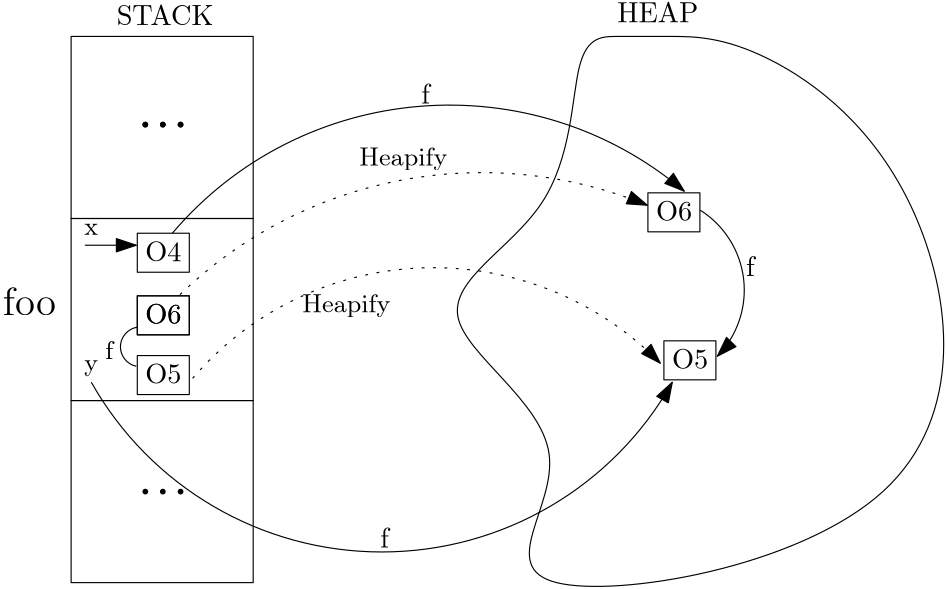
\includegraphics[width=0.9\linewidth]{figures/pldi_6.png}
  \caption{Architecture of PYE (adapted from~\cite{thakur2019pye}). The static side writes
           partial summaries to \texttt{.res} files; the JIT side combines them with library
           summaries to obtain final results.}
  \label{fig:pye}
\end{figure}

These checks are executed on every reference store in optimistically compiled code, so their
cost matters. The third idea of the paper addresses this: the static analysis is also used to
choose the \emph{order} in which objects are laid out on the stack, which reduces the run-time
overhead of the heapification checks.

\subsection{Evaluation}

The authors evaluate their implementation in OpenJ9 on the DaCapo 23.11-Chopin~\cite{blackburn2025rethinking}
and DaCapo 9.12-MR1~\cite{blackburn2006dacapo} benchmark suites and on SPECjvm2008~\cite{specjvm2008}.
Table~\ref{tab:anand-eval} summarizes the improvements they report.

\begin{table}[htbp]
  \centering
  \begin{tabular}{@{}llll@{}}
    \toprule
    Metric & Measured as & Unit & Reported change \\
    \midrule
    Stack allocation & objects allocated on the stack & count & $+71\%$ \\
    Garbage collection & time spent in GC & s & $-5.3\%$ \\
    Performance & execution time & s & $-8.8\%$ \\
    \bottomrule
  \end{tabular}
  \caption{Results reported by Anand et al.~\cite{anand2024optimistic}. More stack allocation means
           fewer heap allocations, which lowers GC time and overall execution time.}
  \label{tab:anand-eval}
\end{table}

\section{Discussion}

These results suggest that stack allocation is worth pursuing further:
\begin{itemize}
  \item it delivers significant performance improvements on real benchmarks;
  \item it is backed by active research that is mature enough to build on but leaves room for
        new contributions, and the baselines and tooling (an OpenJ9 implementation, a static
        analysis, benchmark set-ups) already exist; and
  \item it unlocks further optimization opportunities.
\end{itemize}
Two directions stand out as natural next steps, and they are the subject of our experiments in
Chapter~\ref{ch:experiments}: making smarter use of the fixed stack-frame budget available for
stack-allocated objects, and extending the analysis (static and dynamic) to \emph{arrays}.
